%Chargement des paquets
\usepackage{amsmath}
\usepackage{amsfonts}
\usepackage{amssymb}
\usepackage{enumerate}
\usepackage{mathtools}
\usepackage{bbm}
\usepackage{xparse, etoolbox}
\usepackage{enumerate}
\usepackage{enumitem}
\usepackage{mathabx}
\usepackage{babel}[french]

%environment
\usepackage{amsthm}
\usepackage{keytheorems}
\usepackage{hyperref} 

%Interface théorème
\newkeytheorem{lem}[
	name = Lemme
]

\newkeytheorem{prop}[
	name = Proposition
]

\newkeytheorem{thm}[
	name = Théorème
]

\newkeytheorem{coro}[
	name = Corollaire
]

\renewcommand*{\proofname}{Démonstration}

\theoremstyle{definition}
\newtheorem{defn}{Définition}

\theoremstyle{definition}
\newtheorem*{nota}{Notation}

\theoremstyle{definition}
\newtheorem*{limi}{Liminaire}

\theoremstyle{remark}
\newtheorem{rmq}{Remarque}

\theoremstyle{plain}
\newtheorem*{fait}{Fait}


%Ensembles de nombres
\newcommand{\N} {\mathbb{N}}
\newcommand{\Ne}{\N^\ast}
\newcommand{\Z} {\mathbb{Z}}
\newcommand{\Q} {\mathbb{Q}}
\newcommand{\R} {\mathbb{R}}
\newcommand{\Rb}{\overline{\mathbb{R}}}
\newcommand{\Rp}{\R_+}
\newcommand{\Rm}{\R_-}
\newcommand{\K} {\mathbb{K}}
\newcommand{\Ket} {\mathbb{K^{\ast}}}
\newcommand{\Cx}{\mathbb{C}}

%Ensembles, tribus
\newcommand{\A}{\mathbb{A}}
\renewcommand{\P}{\mathcal{P}}
\newcommand{\T}{\mathcal{T}}
\newcommand{\F}{\mathcal{F}}
\newcommand{\C} {\mathcal{C}}
\newcommand{\ouv}{\mathcal{O}}
\newcommand{\B}{\mathcal{B}}
\newcommand{\M}{\mathcal{M}}
\newcommand{\etag}{\mathcal{E}}
\newcommand{\etagOp}{\etag^{+}(\Omega)}
\newcommand{\etagO}{\etag(\Omega)}
%%Lp avant quotientage
\newcommand{\Lic}{\mathcal{L}^1}
\newcommand{\Lpc}{\mathcal{L}^p}
\newcommand{\Linfc}{\mathcal{L}^{\infty}}
\newcommand{\Lifull}{\Lic(\Omega, \B, m)}
\newcommand{\Lpfull}{\Lpc(\Omega, \B, m)}
\newcommand{\Linffull}{\Linfc(\Omega, \B, m)}
%%Lp après quotientage
\newcommand{\Li}{L^1}
\newcommand{\Ld}{L^2}
\newcommand{\Lp}{L^p}
\newcommand{\Linf}{L^{\infty}}
\newcommand{\Listd}{\Li(\Omega, m)} 
\newcommand{\Ldstd}{\Ld(\Omega, m)} 
\newcommand{\Lpstd}{\Lp(\Omega, m)} 

%Quelques opérateurs
\DeclareMathOperator{\codim}{codim}
\DeclareMathOperator{\rg}{rg}
\DeclareMathOperator{\tr}{tr}
\DeclareMathOperator{\vect}{Vect}
\DeclareMathOperator{\ima}{Im}
\DeclareMathOperator{\id}{Id}
\DeclareMathOperator{\sign}{sign}
\DeclareMathOperator{\ext}{ext}
\newcommand{\ind}{\mathbbm{1}}
\newcommand*{\spr}[2]{\left(\,#1\,\middle|\,#2\,\right)}
\newcommand{\interior}[1]{%
  {\kern0pt#1}^{\mathrm{o}}%
}
\DeclareMathOperator{\card}{card}
\DeclareMathOperator{\ppcm}{ppcm}

%Commandes de pure flemme
\newcommand{\veps}{\varepsilon}
\newcommand{\intab}{\int_{a}^{b}}
\newcommand{\intR}{\int_{-\infty}^{\infty}}
\newcommand{\intinf}{\int_{- \infty}^{+ \infty}}
\newcommand{\equi}{\Leftrightarrow}
\newcommand{\Kev}{$\K$-espace vectoriel }
\newcommand{\Kevs}{$\K$-espaces vectoriels }
\newcommand{\Rev}{$\R$-espace vectoriel }
\newcommand{\Revs}{$\R$-espaces vectoriels }
\newcommand{\Cev}{$\Cx$-espace vectoriel }
\newcommand{\Cevs}{$\Cx$-espaces vectoriels }
\newcommand{\evn}{(E, \norm{.})}
\newcommand{\interf}[2]{[#1,#2]}
\newcommand{\limb}{\lim\limits_}
\newcommand{\lebn}{\lambda_n}
\newcommand{\pp}{\text{~presque partout}}
\newcommand{\derivp}[2]{\frac{\partial #1}{\partial #2}}
\newcommand{\famiu}{(u_i)_{i \in I}}
\newcommand{\sev}{\text{~s.e.v.}}
\newcommand{\Mnp}{M_{n,p}(\K)}
\newcommand{\Mn}{M_{n}(\K)}
\newcommand{\tq}{\text{~t.q.~}}
\newcommand{\mq}{~montrer~que~}
\newcommand{\et}{\quad \text{et} \quad}
\newcommand{\ou}{\text{~ou~}}
\newcommand{\Kx}{\K[X]}


%Commandes de gars chelou
\renewcommand{\subset}{\subseteq}

%Commande restriction, ty duckduckgo
\def\restr#1#2{\mathchoice
              {\setbox1\hbox{${\displaystyle #1}_{\scriptstyle #2}$}
              \restraux{#1}{#2}}
              {\setbox1\hbox{${\textstyle #1}_{\scriptstyle #2}$}
              \restraux{#1}{#2}}
              {\setbox1\hbox{${\scriptstyle #1}_{\scriptscriptstyle #2}$}
              \restraux{#1}{#2}}
              {\setbox1\hbox{${\scriptscriptstyle #1}_{\scriptscriptstyle #2}$}
              \restraux{#1}{#2}}}
\def\restraux#1#2{{#1\,\smash{\vrule height .8\ht1 depth .85\dp1}}_{\,#2}} 

%Quelques normes
\DeclarePairedDelimiter\abs{\lvert}{\rvert}
\DeclarePairedDelimiter\labs{\bigl\lvert}{\bigr\rvert}
\DeclarePairedDelimiter\norm{\lVert}{\rVert}
\DeclarePairedDelimiterXPP\normi[1]{}\lVert\rVert{_1}{\ifblank{#1}{\:\cdot\:}{#1}}
\DeclarePairedDelimiterXPP\normd[1]{}\lVert\rVert{_2}{\ifblank{#1}{\:\cdot\:}{#1}}
\DeclarePairedDelimiterXPP\normp[1]{}\lVert\rVert{_p}{\ifblank{#1}{\:\cdot\:}{#1}}
\DeclarePairedDelimiterXPP\normq[1]{}\lVert\rVert{_q}{\ifblank{#1}{\:\cdot\:}{#1}}
\DeclarePairedDelimiterXPP\norminf[1]{}\lVert\rVert{_\infty}{\ifblank{#1}{\:\cdot\:}{#1}}

%Bracket en angle
\DeclarePairedDelimiter\angl{\langle}{\rangle}

%Set, parenthèses
\newcommand{\set}[1]{\{ #1 \}}
\newcommand{\bigset}[1]{\bigl\{ #1 \bigr\}}
\newcommand{\Bigset}[1]{\Bigl\{ #1 \Bigr\}}
\newcommand{\bigpar}[1]{\bigl( #1 \bigr)}
\newcommand{\Bigpar}[1]{\Bigl( #1 \Bigr)}

%Opitmisation des opérateurs de comparaison
\DeclarePairedDelimiter\tio{o (}{)}
\DeclarePairedDelimiter\gro{O (}{)}

\usetikzlibrary{patterns,arrows.meta}

\pagestyle{fancy}

\fancyhead[C]{Le lemme de la Grenouille}
\fancyhead[R]{}

\begin{document}

\underline{Sources :} 
\begin{itemize}
\item Gourdon - Analyse - exercice 7 page 46 (le lemme).
\item S. Francinou, H. Gianella et S. Nicolas - Oraux X-ENS (l'application).
\end{itemize}

\underline{Leçons :}
\begin{itemize}

\item 203 : Utilisation de la notion de compacité.
\item 223 : Suites réelles et complexes. Convergence, valeurs d’adhérence. Exemples et applications.
\item 226 : Suites vectorielles et réelles définies par une relation de récurrence $u_{n+1}=f(u_n)$. Exemples. 
Applications à la résolution approchée d’équations.
\item 204 : Connexité. Exemples d’applications.

\end{itemize}

\begin{lem}
Soit $(E,d)$ un espace métrique compact et $(u_n)_\N$ une suite de $E$ telle que $\lim_{n\to\infty} d(u_n,u_{n+1}) = 0$.
Alors, l'ensemble des valeurs d'adhérence de $(u_n)_\N$ est connexe.
\end{lem}

\begin{proof}
Pour tout $p \in \N$, on note $A_p= \set{u_n, n \geq p}$. 
On note aussi $\Gamma$ l'ensemble des valeurs d'adhérence de la suite $(u_n)_\N$.
On peut démontrer que $\Gamma = \bigcap_{p \in \N} \overline{A_p}$ (de façon informelle si $l$ valeur d'adhérence, 
alors pour une distance arbitraire et un rang arbitraire, 
il existe un terme de la suite d'au moins ce rang et distant d'au plus cette distance de la valeur d'adhérence).
En particulier, $\Gamma$ est un fermé de $E$, et comme $E$ est compact, $\Gamma$ l'est aussi. \newline
Supposons que $\Gamma$ ne soit pas connexe, de sorte que l'on puisse écrire $\Gamma = A \cup B$ avec $A$ et $B$ deux fermés disjoints non vides.
Comme $A$ et $B$ sont éléments de $E$, ils sont aussi compacts.
Par continuité de l'application $d : (x,y) \mapsto d(x,y)$ sur le compact $A \times B$, il existe un couple $(a,b) \in A \times B$ telle que 
$d$ atteigne son minimum sur $A \times B$. Comme $A$ et $B$ sont disjoints, ce minimum est strictement positif.
Ainsi, $\alpha = d(A,B) >0$, et on note :
\[ A'  = \Bigset{x \in E ; d(x,A) < \dfrac{\alpha}3} = \bigcup_{x \in A} B\Bigpar{x, \dfrac{\alpha}3} \et
	B'  = \Bigset{x \in E ; d(x,B) < \dfrac{\alpha}3} = \bigcup_{x \in B} B\Bigpar{x, \dfrac{\alpha}3} . \]
	
	
\begin{center}

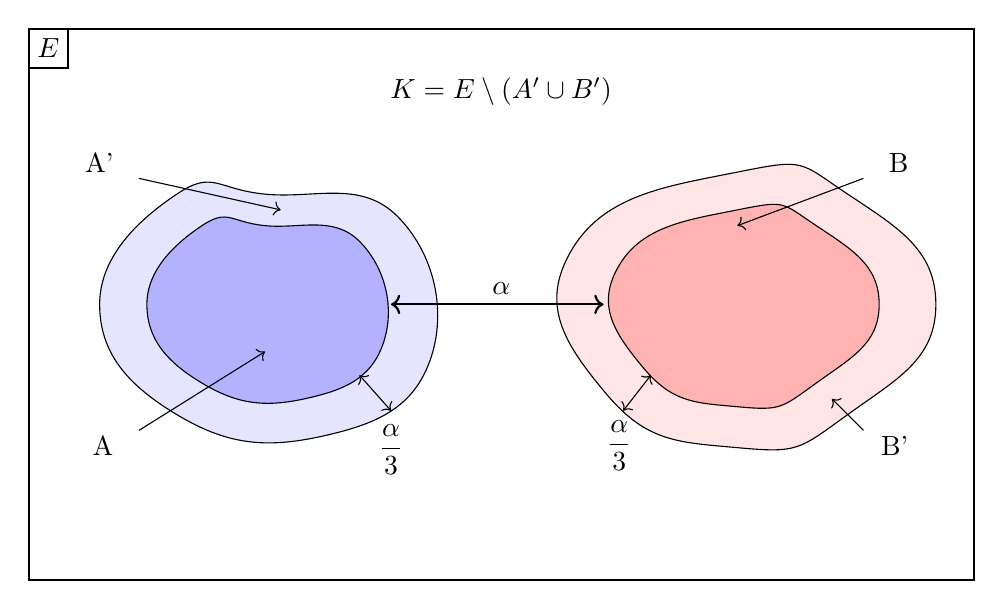
\begin{tikzpicture}

% --- Rectangle containers ---
\draw[thick] (-6,-3.5) rectangle (6,3.5);
\draw[thick] (-6,3.5) rectangle (-5.5,3);

% --- Label ---
\node[below] at (0,3) {$K= E \setminus (A' \cup B')$};
\node at (-5.75, 3.25) {$E$};

% --- Define Blob Shape 1 ---
\def\blobA{
  plot[smooth cycle, tension=0.8] coordinates {
    (0,1) (1.2,0.8) (1.5,-0.5) (0.5,-1.2)
    (-0.8,-1) (-1.5,0) (-0.8,1)
  }
}

% --- Left pair (Blob 1 inside Blob 2) ---
\begin{scope}[shift={(-3,0)}, scale=1.4]
\draw[fill=blue!10] \blobA; % Blob 2 (outer)
\end{scope}

\begin{scope}[shift={(-3,0)}, scale=1]
\draw[fill=blue!30] \blobA; % Blob 1 (inner)
\end{scope}

% Labels for left pair
\node[left] at (-4.8,-1.8) {A};
\draw[->] (-4.6,-1.6) -- (-3,-0.6); % points to inner blob

\node[left] at (-4.8,1.8) {A'};
\draw[->] (-4.6,1.6) -- (-2.8,1.2); % points to outer blob

% Arrow between left blobs
\node[below] at (-1.4,-1.4) {$\dfrac{\alpha}3$};
\draw[<->] (-1.8, -0.9) -- (-1.4, -1.35);

% --- Define Blob Shape 3 ---
\def\blobB{
  plot[smooth cycle, tension=0.9] coordinates {
    (0,1.2) (1,1) (1.8,0) (1,-1)
    (0,-1.3) (-1.2,-0.8) (-1.5,0.5)
  }
}

% --- Right pair (Blob 3 inside Blob 4) ---
\begin{scope}[shift={(3,0)}, scale=1.4]
\draw[fill=red!10] \blobB; % Blob 4 (outer)
\end{scope}

\begin{scope}[shift={(3,0)}, scale=1]
\draw[fill=red!30] \blobB; % Blob 3 (inner)
\end{scope}

% Labels for right pair
\node[right] at (4.8,1.8) {B};
\draw[->] (4.6,1.6) -- (3,1); % points to outer blob

\node[right] at (4.7,-1.8) {B'};
\draw[->] (4.6,-1.6) -- (4.2,-1.2); % points to inner blob

% Arrow between right blobs
\node[below] at (1.5, -1.35) {$\dfrac{\alpha}3$};
\draw[<->] (1.9, -0.9) -- (1.55, -1.35);

% Arrow between outer blobs
\node[above] at (0,0) {$\alpha$};
\draw[<->, thick] (-1.4,0) -- (1.3,0);


\end{tikzpicture}

\end{center}
Il est important de noter que les ensembles $A'$ et $B'$ sont disjoints (sinon il existerait $(a,b) \in A \times B$ tel que $d(a,b) < \alpha$).
De plus, es ensembles $A'$ et $B'$ sont des ouverts donc $K = E \setminus (A' \cup B')$ est fermé dans le compact $E$, 
donc est compact.
Nous allons montrer que la suite $(u_n)_\N$ admet une valeur d'adhérence dans $K$, 
ce qui est absurde car $\Gamma \cap K = \emptyset$. \\
Comme $\lim_{n \to \infty} d(u_n,u_{n+1}) = 0$, on a :
\[ \exists N_0 \in \N, \forall n \in \N : n \geq N_0 \Rightarrow d(u_n, u_{n+1}) < \dfrac{\alpha}3 . \qquad (*) \]
Prenons $N \geq N_0$ et $x_0 \in A$. Comme $x_0$ est une valeur d'adhérence de $(u_n)_\N$, il existe un entier $n_1 \geq N$ tel que 
$d(u_{n_1}, x_0) < \alpha /3$ donc $u_{n_1} \in A'$. 
Prenons maintenant $y_0 \in B$, de même, $y_0$ est une valeur d'adhérence de $(u_n)_\N$, il existe donc un entier $n_3 > n_1$ 
tel que $d(u_{n_3}, y_0 < \alpha/3$, de sorte que $u_{n_3} \in B'$.
Notons $n_2$ le plus petit entier supérieur à $n_1$ et tel que $u_{n_2} \not \in A'$. Cet entier existe car $u_{n_3} \in B'$. 
On a $u_{n_2-1} \in A'$ donc, d'après la relation (*) :
\[ d(u_{n_2}, B) \geq d(u_{n_2-1}, B) - d(u_{n_2-1}, u_{n_2}) \geq d(A,B) - d(u_{n_2-1}, A) - d(u_{n_2-1}, u_{n_2}) > \dfrac{\alpha}3 , \]
ce qui prouve que $u_{n_2} \not \in B'$. Comme de plus,  $u_{n_2} \not \in A'$, on a  $u_{n_2} \in K$. \\
Ceci étant valable pour tout entier $N \geq N_0$, on peut ainsi construire une suite extraite de $(u_n)_\N$ à valeurs dans $K$.
Et $K$ étant compact, cette suite admettra nécessairement une valeur d'adhérence dans $K$, donc la suite $(u_n)_\N$ admet une 
valeur d'adhérence dans $K$, et on arrive à la contradiction recherchée.
\end{proof}

\begin{appl}
Si $f : [0,1] \to [0,1]$ est continue, alors la suite définie par :
\[ u_0 \in [0,1] \et u_{n+1} = f(u_n) , \]
converge si, et seulement si, $u_{n+1}-u_n$ converge vers 0.
\end{appl}

\begin{proof}
La condition nécessaire est claire, il reste donc à montrer la condition suffisante. Supposons que $u_{n+1}-u_n$ converge vers 0
mais que la suite $(u_n)_\N$ ne converge pas. Par compacité de $[0,1]$, la suite admet au moins deux valeurs d'adhérence distincte
$l < l'$ toutes deux dans $[0,1]$. 
Or, pour toute valeur d'adhérence $a \in [0,1]$ de $(u_n)_\N$, en notant $\psi$ une fonction extractrice sur $\N$ 
tel que $(u_{\psi(n)})_\N$ converge vers $a$, on a, par continuité de $f$ en $a$ :
\[ a = \lim_{n \to \infty} u_{\psi(n)+1} = \lim_{n \to \infty} f(u_{\psi(n)} = f(a) . \]
Autrement dit, toute valeur d'adhérence de $(u_n)_\N$ est un point fixe de $f$. 
Or, selon le lemme de la grenouille, l'ensemble $\Gamma$ des valeurs d'adhérence de $(u_n)_\N$ est un connexe de $\R$, 
et donc $[l, l'] \subset \Gamma$.
En particulier, $\dfrac{l+l'}2$ est une valeur d'adhérence de $(u_n)_\N$, il existe donc un rang $p \in \N$ tel que :
\[ \abs*{u_p - \dfrac{l+l'}2} \leq \dfrac{l'-l}2 , \]
autrement dit, $u_p \in [l, l'] \subset \Gamma$ si bien que la suite $(u_n)_\N$ est stationnaire à partir du rang $p$, donc convergente,
ce qui est contradictoire. La condition suffisante est donc démontrée.
\end{proof}

\end{document}